\section{Measuring \textit{in vivo} turnover rates with smPReSS}

In order to better understand the role of , we needed to have a way to .  One alternative would have been use .  

\subsection{smPReSS measurement technique}

Copy and paste from paper when I have access

\begin{figure}[h!]
\centering
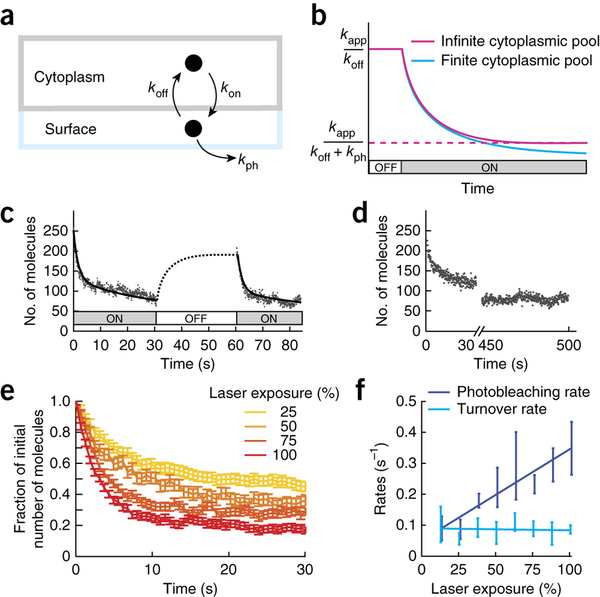
\includegraphics[width=0.8\hsize]{nmeth/nmeth.jpg}
\caption{smPReSS measurement technique.  \textbf{a)}  The basic kinetic principle: during imaging, the level of surface-associated proteins is set by a dynamic balance of appearance (binding or assembly) at an observable rate $k_{app}$, disappearance (unbinding or disassembly) at a per-molecule rate $k_{off}$, and photobleaching at a per-molecule rate $k_{ph}$.  \textbf{b)} Predicted response of an initially unobserved cell at steady state to a step change in illumination. For an infinite cytoplasmic pool, the surface density relaxes to a new illuminated steady state. For a finite cytoplasmic pool, fast relaxation is accompanied by a slower decay caused by irreversible photobleaching. \textbf{c)} Fast relaxation to a quasi-stable density during illumination is rapidly reversed when the laser is turned off. \textbf{d)}  Biphasic response for GFP::actin under illumination conditions that allow accurate single-molecule detection and tracking. Time from $t$ = 30-450 s is discontinuous. \textbf{e)} Surface density of GFP::actin vs. time at various laser exposures, shown as a fraction of the initial unobserved density. Error bars, s.e.m. ($n$ = 7, 9, 6, 7 embryos for laser exposures from low to high). textbf{f)} Estimates of per-molecule turnover ($k_{off}$) and photobleaching ($k_{ph}$) rates as a function of laser exposure. Error bars, s.d. (n = 12, 7, 8, 9, 7, 6, 7, 7 embryos, low to high laser exposure). Solid lines show a linear regression against the data. 100\% laser power $\approx 1.6 \mu W/\mu m^2$.} 
 
\end{figure}


\subsection{Measurements of turnover rate in dividing \textit{C. elegans} cortex}

Copy and paste from paper when I have access

\begin{figure}[h!]
	\centering
	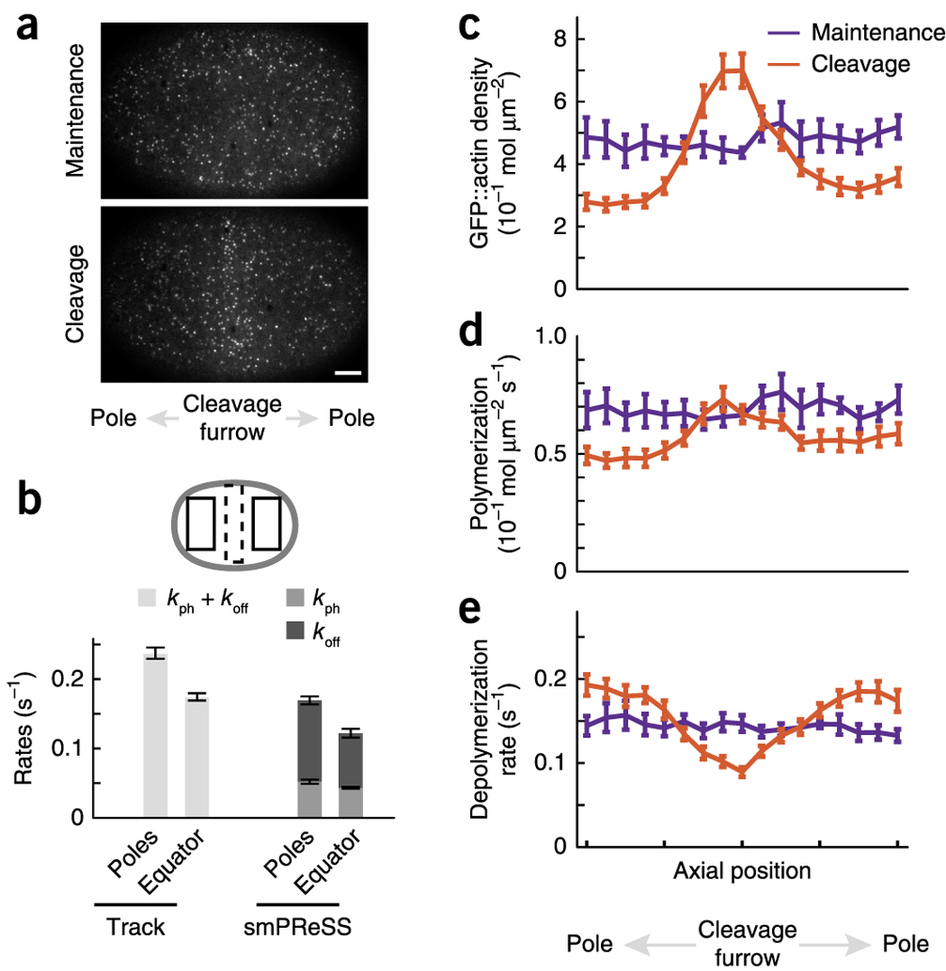
\includegraphics[width=0.8\hsize]{nmeth/nmethF4.jpg}
	\caption{Measurement of cortical actin lifetimes.  \textbf{a)} Near-TIRF micrographs of GFP::actin during the polarity maintenance phase (top) and cleavage (bottom). \textbf{b)} Measurements of the indicated turnover rates at the equator and poles during anaphase using tracking (left) or smPReSS (right). Schematic indicates the equatorial (dashed box) and polar (solid boxes) regions in which the measurements were made. For tracking, the sum of koff and kph is displayed; for smPReSS, the values for $k_{ph}$ and $k_{off}$ are stacked. \textbf{c-e)} Spatial variation in actin density and turnover kinetics during maintenance phase and cleavage measured by tracking and binned along the antero-posterior axis. \textbf{c)} Cortical density. \textbf{d)} Polymerization rate. \textbf{e)} Depolymerization rate (instantaneous disappearance rate minus estimated photobleaching rate). In b-e, error bars indicate cell-to-cell s.e.m. (n = 7 embryos, maintenance, and n = 16 embryos, cleavage). Scale bar, $5 \mu m$.} 
	
\end{figure}

